\begin{Centrage}
	\textbf{Partie A : étude de la fonction $\bm{f}$.}
\end{Centrage}

La fonction $f$ est définie sur l'intervalle $\IntervalleOO{0}{+\infty}$ par : $f(x)=x-2+\frac{1}{2} \ln(x)$, où $\ln$ désigne la fonction logarithme népérien.

On admet que la fonction $f$ est deux fois dérivable sur $\IntervalleOO{0}{+\infty}$, on note $f^{\prime}$ sa dérivée et $f^{\prime\prime}$ sa dérivée seconde.

\begin{enumerate}
	\item 
	\begin{enumerate}
		\item Déterminer, en justifiant, les limites de $f$ en $0$ et en $+\infty$.
		\item Montrer que pour tout $x$ appartenant à $\IntervalleOO{0}{+\infty}$, on a : $f^{\prime}(x)=\frac{2x+1}{2x}$.
		\item Étudier le sens de variation de $f$ sur $\IntervalleOO{0}{+\infty}$.
		\item Étudier la convexité de $f$ sur $\IntervalleOO{0}{+\infty}$.
	\end{enumerate}
	\item 
	\begin{enumerate}
		\item Montrer que l'équation $f(x)=0$ admet dans $\IntervalleOO{0}{+\infty}$ une solution unique qu'on notera $\alpha$ et justifier que $\alpha$ appartient à l'intervalle $\IntervalleFF{1}{2}$.
		\item Déterminer le signe de $f(x)$ pour $x \in \IntervalleOO{0}{+\infty}$.
		\item Montrer que $\ln (\alpha)=2(2-\alpha)$.
	\end{enumerate}
\end{enumerate}

\begin{Centrage}
	\textbf{Partie A : étude de la fonction $\bm{g}$.}
\end{Centrage}

La fonction $g$ est définie sur $\IntervalleOF{0}{1}$ par $g(x)=-\frac{7}{8}x^{2}+x-\frac{1}{4} x^{2}\,\ln(x)$.

On admet que la fonction $g$ est dérivable sur $\IntervalleOF{0}{1}$ et on note $g^{\prime}$ sa fonction dérivée.

\begin{enumerate}
	\item Calculer $g^{\prime}(x)$ pour $x \in \IntervalleOF{0}{1}$ puis vérifier que $g^{\prime}(x)=x\,{f\left(\frac{1}{x}\right)}$.
	\item 
	
	\begin{enumerate}
		\item Justifier que pour $x$ appartenant à l'intervalle $\IntervalleOO{0}{\frac{1}{\alpha}}$, on a $f{\left(\frac{1}{x}\right)}>0$.
		\item On admet le tableau de signes suivant :
		
		\begin{Centrage}
			\begin{tikzpicture}[double distance=2pt]
				\tkzTabInit[lgt=4]{$x$/1,Signe de $f{\left(\frac{1}{x}\right)}$/1.15}{$0$,$\frac{1}{\alpha}$,$1$}
				\tkzTabLine{d,+,z,-,}
			\end{tikzpicture}
		\end{Centrage}
		
		En déduire le tableau de variations de $g$ sur l'intervalle $\IntervalleOF{0}{1}$. Les images et les limites ne sont pas demandées.
	\end{enumerate}
\end{enumerate}

\begin{Centrage}
	\textbf{Partie C : un calcul d'aire.}
\end{Centrage}

On a représenté sur le graphique ci-dessous :

\begin{itemize}
	\item la courbe $\mathcal{C}_{g}$ de la fonction $g$ ;
	\item la parabole $\mathcal{P}$ d'équation $y=-\frac{7}{8}x^{2}+x$ sur l'intervalle $\IntervalleOF{0}{1}$.
\end{itemize}

\begin{Centrage}
	\begin{GraphiqueTikz}[x=12cm,y=12cm,Xmin=0,Xmax=1.05,Xgrille=0.1,Xgrilles=0.1,Ymin=0,Ymax=0.425,Ygrille=0.1,Ygrilles=0.1]
		\def\solalpha{1.72685}
		\TracerAxesGrilles[Grads=false]{auto}{auto}
		\RajouterValeursAxeX{0,0.1,1}{0,\num{0.1},1}
		\RajouterValeursAxeY{0,0,0.1}{0,0,\num{0.1}}
		\DefinirCourbe[Nom=cg,Debut=0.001,Fin=1]<fctg>{-7/8*x^2+x-1/4*x^2*log(x)}
		\DefinirCourbe[Nom=p,Debut=0.001,Fin=1]<fctp>{-7/8*x^2+x}
		\TracerIntegrale[Type=fct/fct,Style=hachures,Couleurs=darkgray]{fctg(x)}[fctp(x)]{1/\solalpha}{1}
		\TracerCourbe[Couleur=blue,Debut=0.001,Fin=1]{fctg(x)}
		\TracerCourbe[Couleur=red,Debut=0.001,Fin=1]{fctp(x)}
		\DefinirImage[Nom=IMGg]{fctg}{1/\solalpha}
		\DefinirImage[Nom=IMGun]{fctg}{1}
		\draw[thick,darkgray,densely dashed] (IMGg) -- ({1/\solalpha},0) node[below] {$\frac{1}{\alpha}$} ;
		\draw[thick,darkgray,densely dashed] (IMGun) --(1,0) ;
		\draw[blue] (0.725,0.333) node[font=\large] {$\mathcal{C}_{g}$} ;
		\draw[red] (0.725,0.233) node[font=\large] {$\mathcal{P}$} ;
	\end{GraphiqueTikz}
\end{Centrage}

On souhaite calculer l'aire $\mathcal{A}$ du domaine hachuré compris entre les courbes $\mathcal{C}_{g}$ et $\mathcal{P}$, et les droites d'équations $x=\frac{1}{\alpha}$ et $x=1$.

On rappelle que $\ln (\alpha)=2(2-\alpha)$.

\begin{enumerate}
	\item 
	
	\begin{enumerate}
		\item Justifier la position relative des courbes $\mathcal{C}_{g}$ et $\mathcal{P}$ sur l'intervalle $\IntervalleOF{0}{1}$.
		\item Démontrer l'égalité : \[ \int_{\frac{1}{\alpha}}^{1} x^2\,\ln(x) \dx = \frac{-\alpha^3-6\alpha+13}{9\alpha^3}. \]
	\end{enumerate}
	\item En déduire l'expression en fonction de $\alpha$ de l'aire $\mathcal{A}$.
\end{enumerate}